\begin{figure}
	\centering
	\begin{subfigure}{0.8\linewidth}
		\centering
		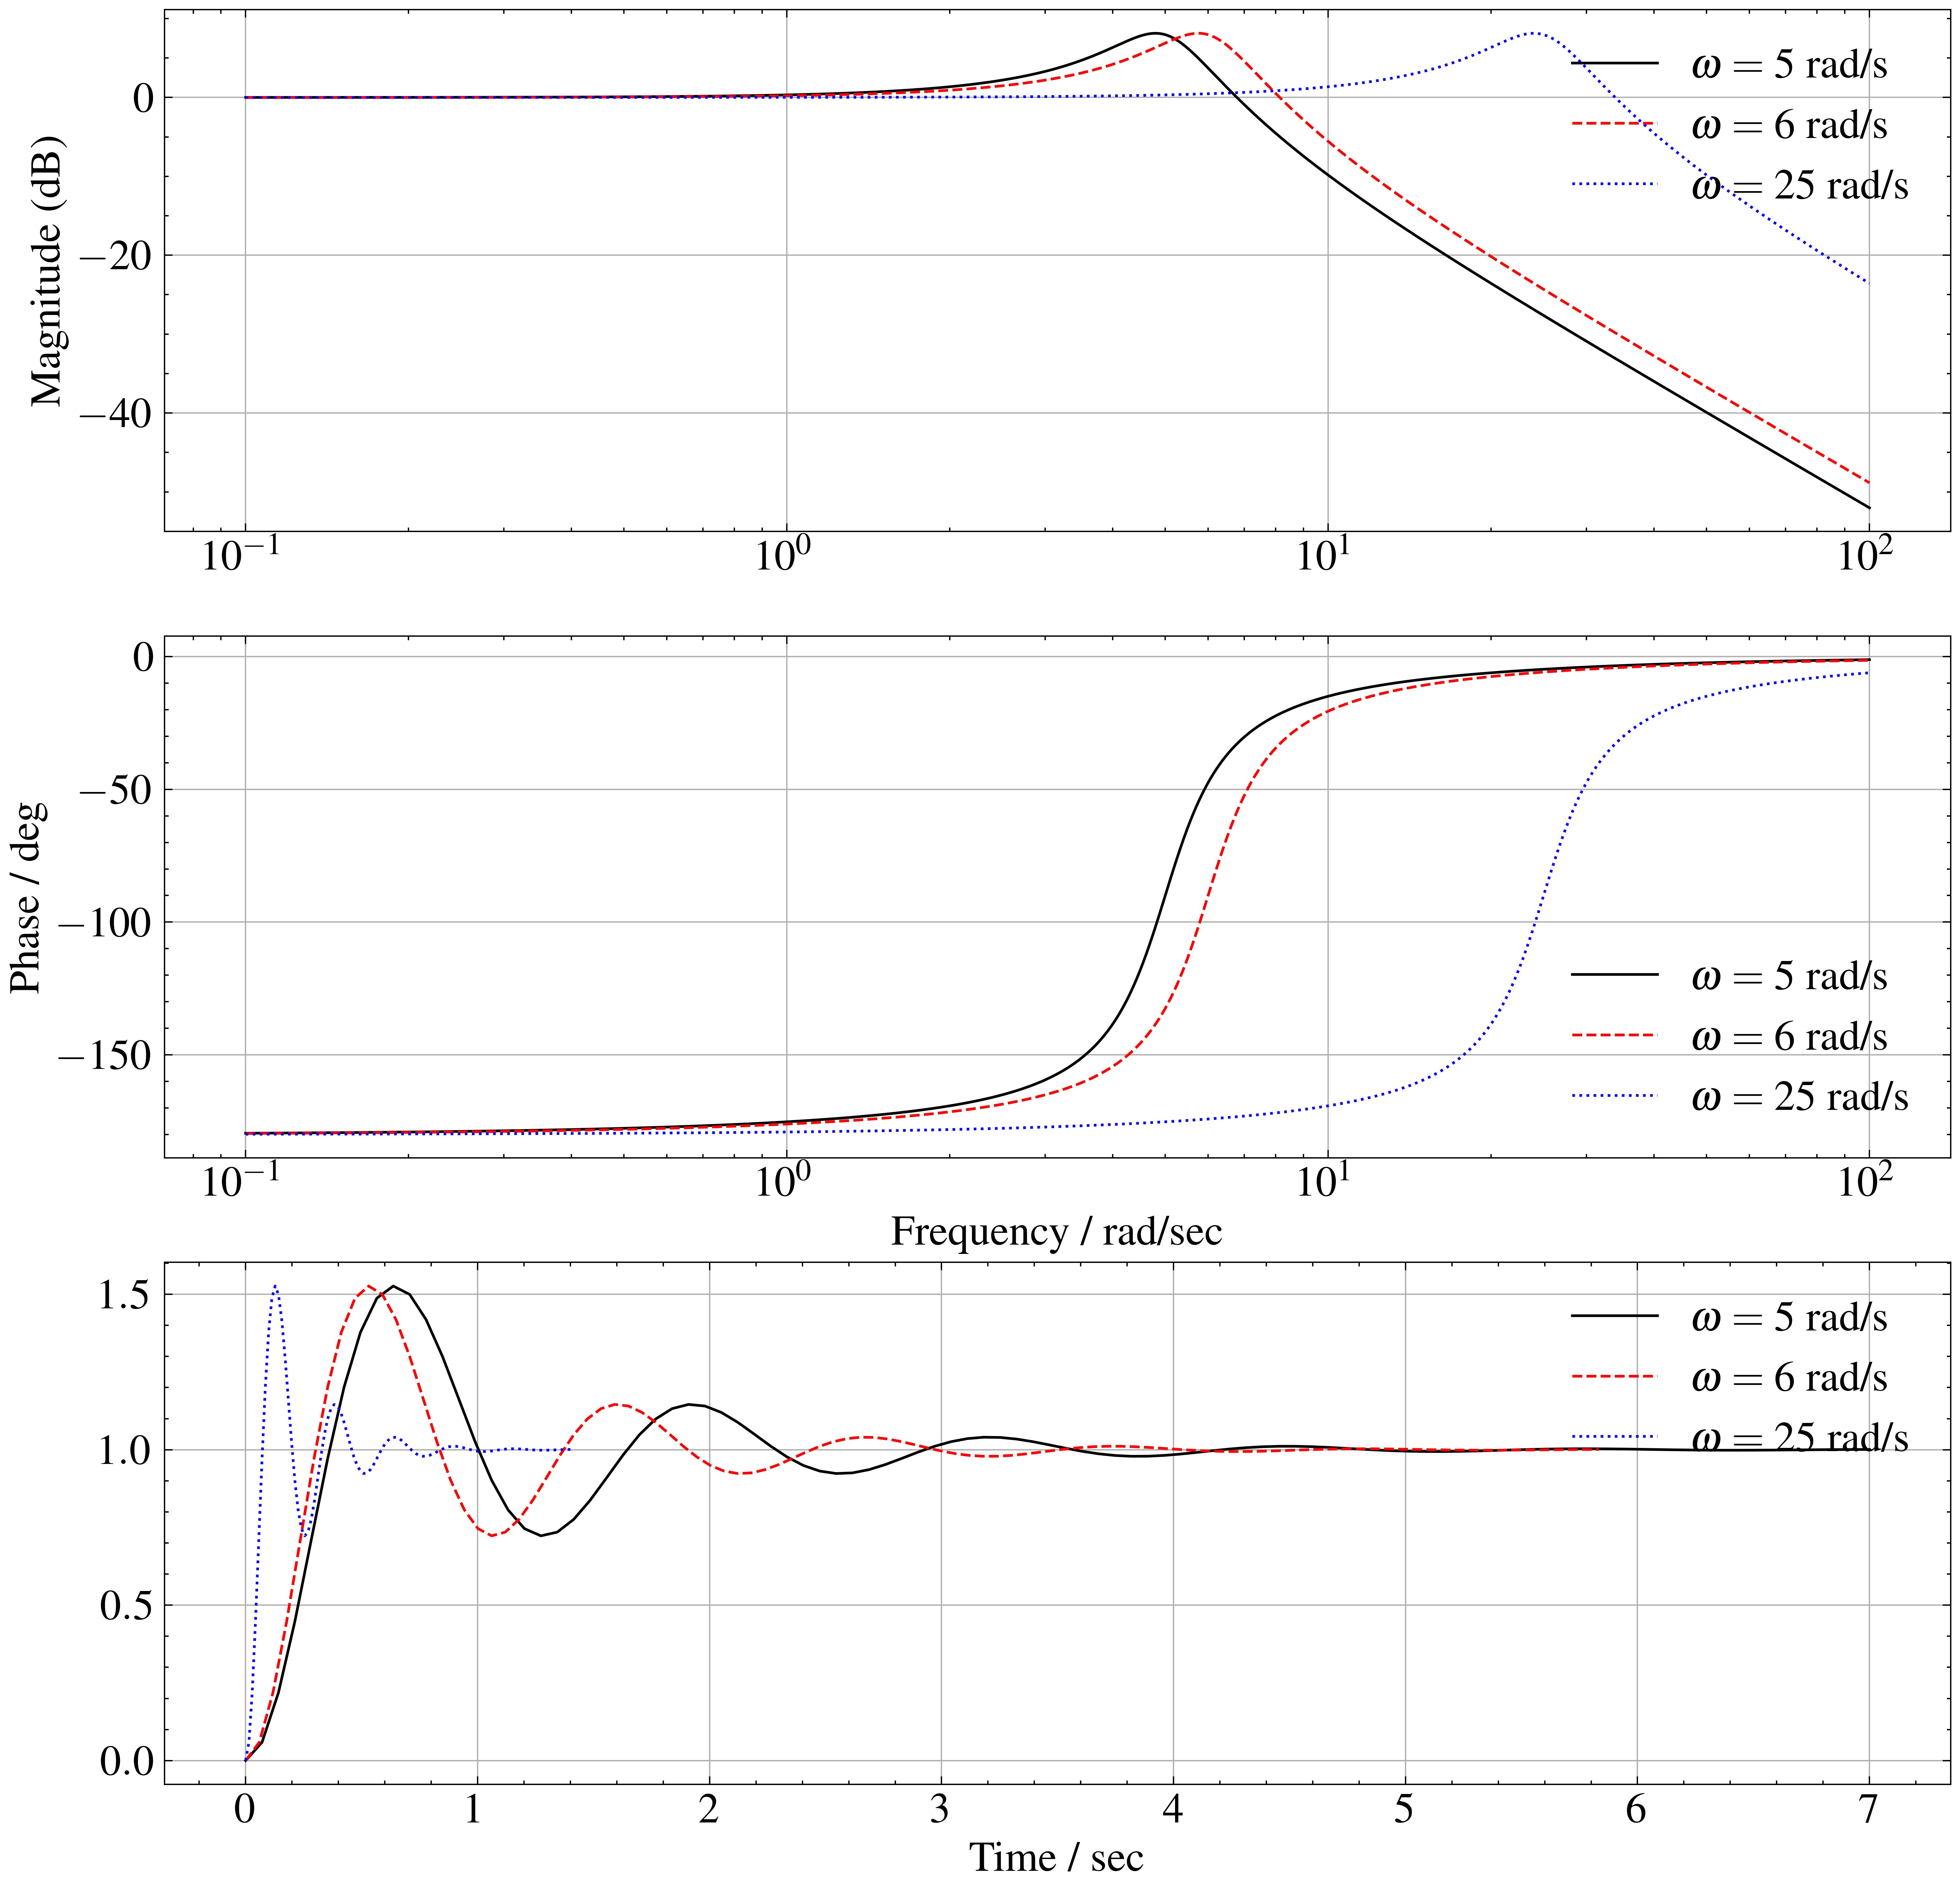
\includegraphics[width=0.8\linewidth]{src/figures/bode-phase-step-ideal-group-zeta/bode-phase-step-ideal-group-zeta-0.2.png}
		\subcaption{$\zeta = 0.2$}\label{fig:bode-phase-step-ideal-group-zeta-0.2}
	\end{subfigure}
	\begin{subfigure}{0.8\linewidth}
		\centering
		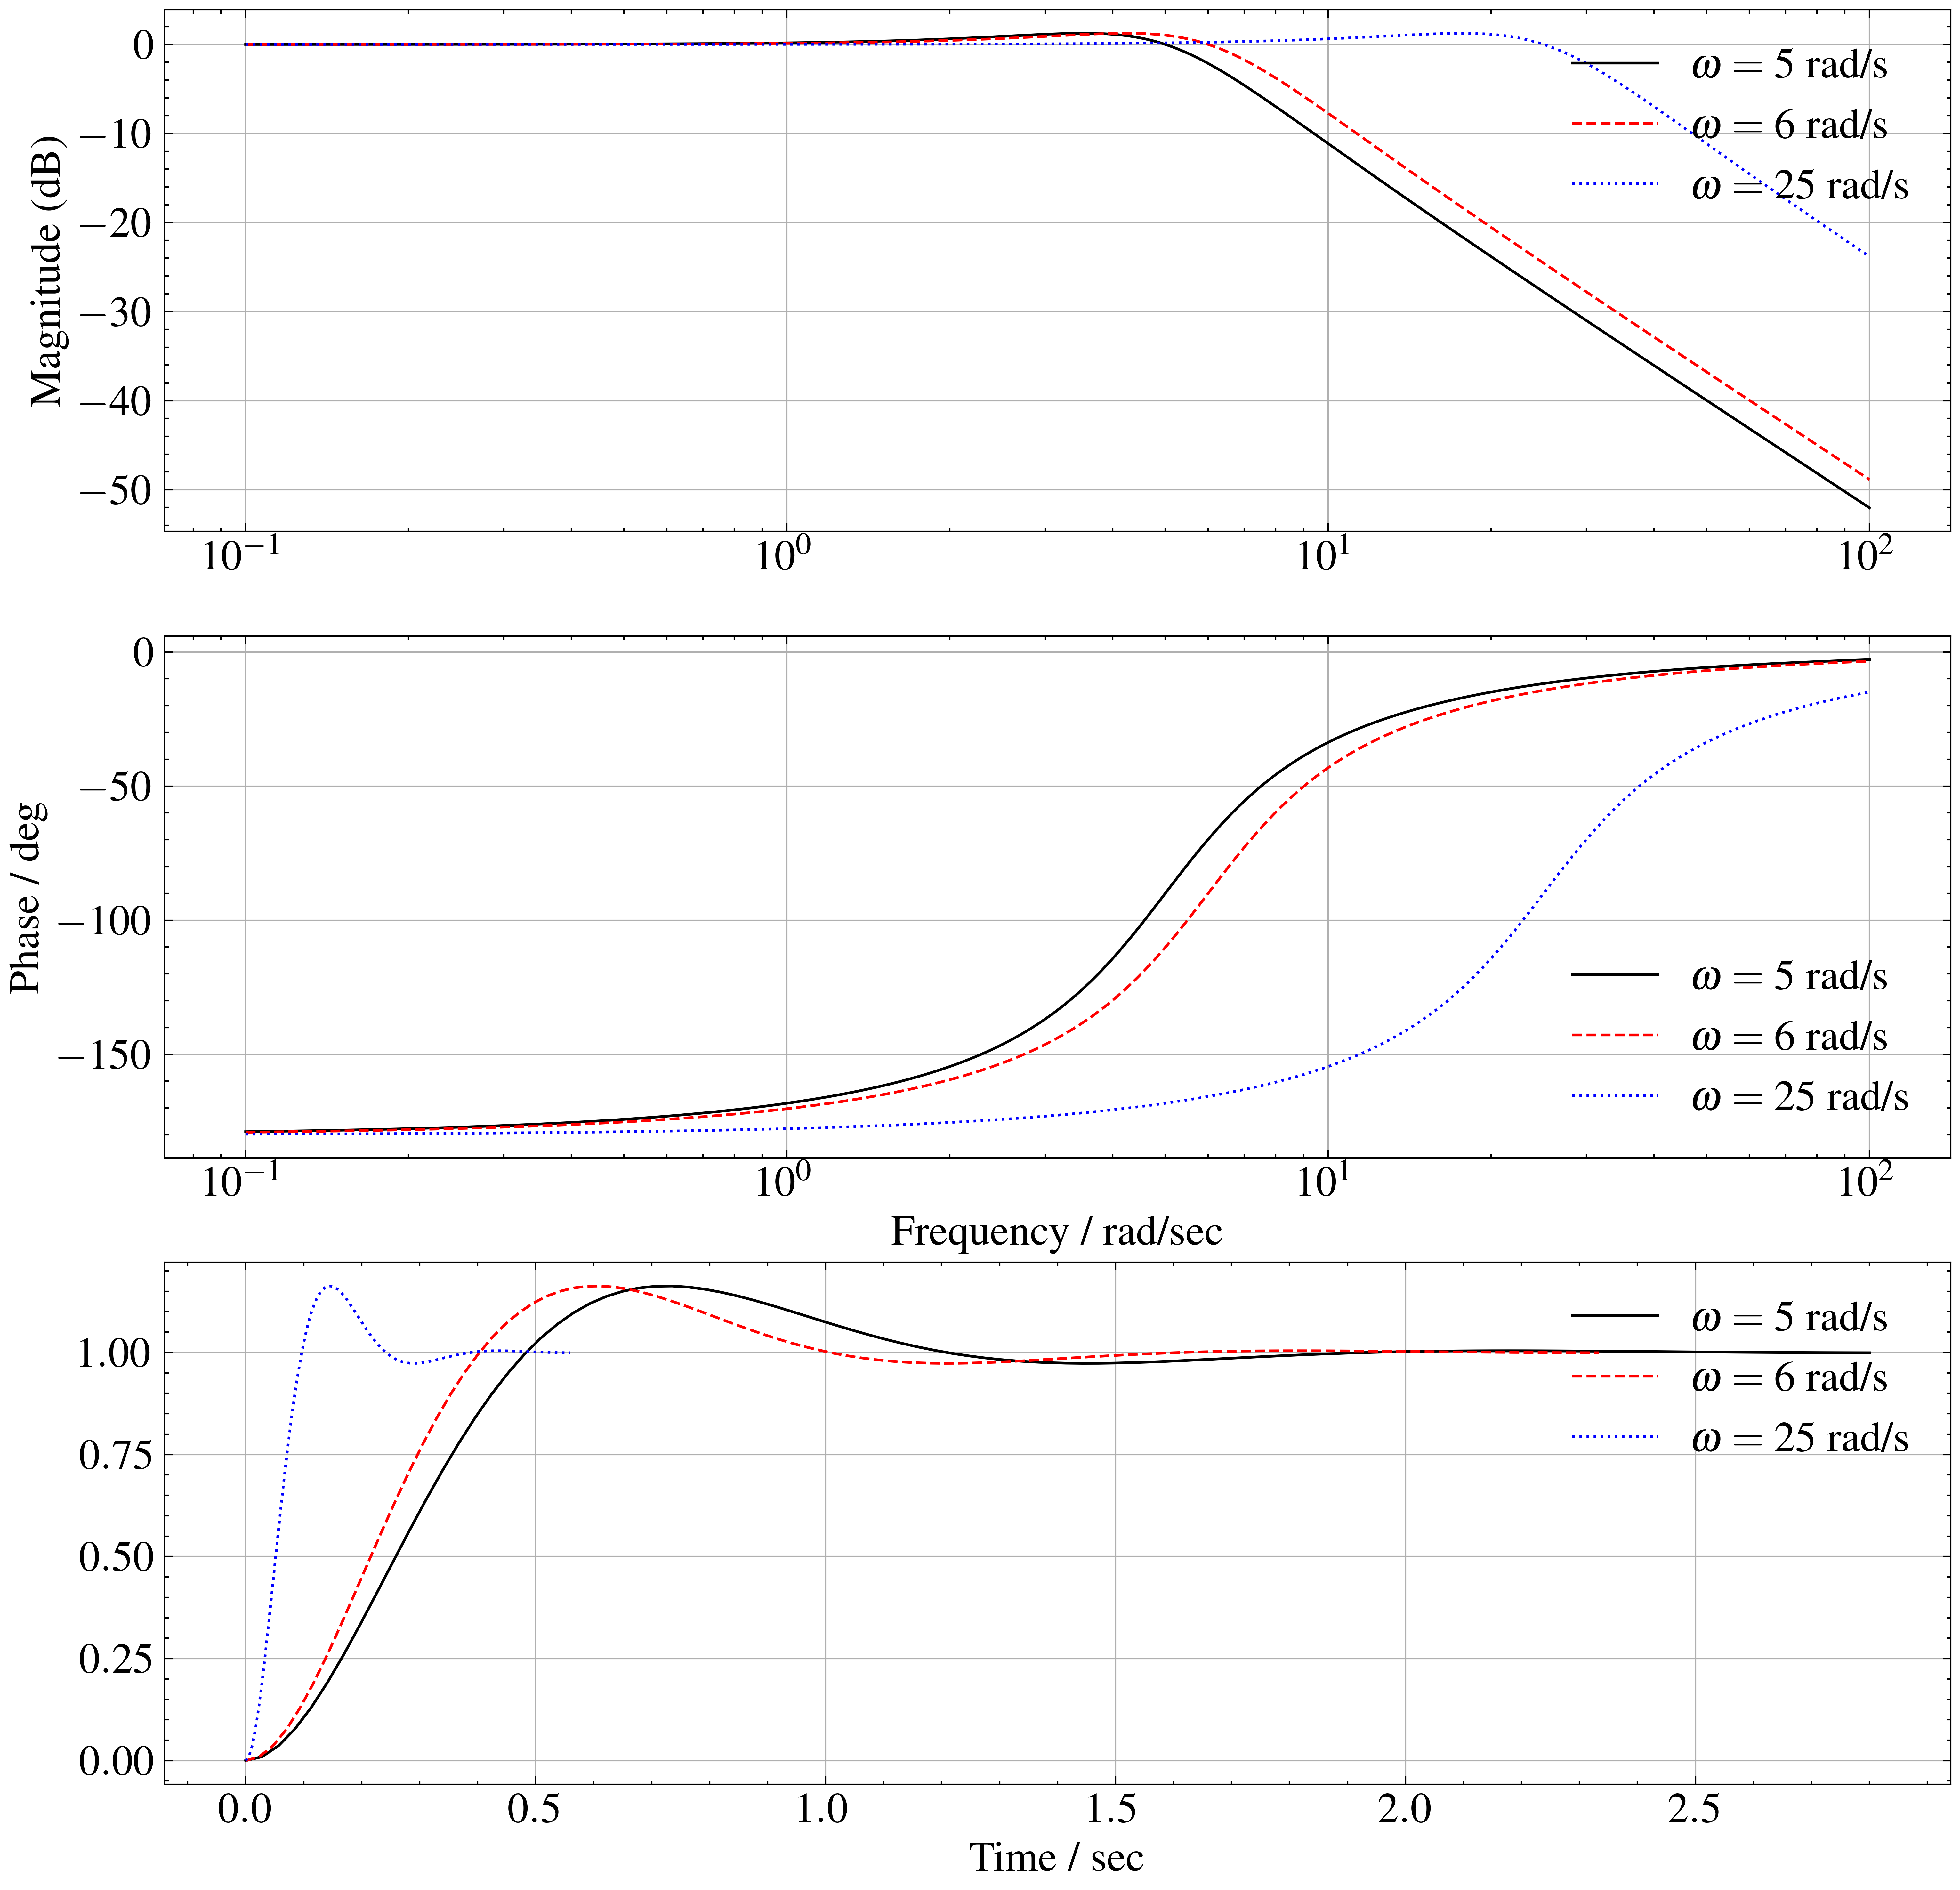
\includegraphics[width=0.8\linewidth]{src/figures/bode-phase-step-ideal-group-zeta/bode-phase-step-ideal-group-zeta-0.5.png}
		\subcaption{$\zeta = 0.5$}\label{fig:bode-phase-step-ideal-group-zeta-0.5}
	\end{subfigure}
	\caption{ある$\zeta$に対して、$\omega$を変化させたときのボード線図とステップ応答}\label{fig:bode-phase-step-ideal-group-zeta}
\end{figure}

\begin{figure}
	\centering
	\addtocontents{figure}{-1}
	\begin{subfigure}{0.8\linewidth}
		\setcounter{subfigure}{2}
		\centering
		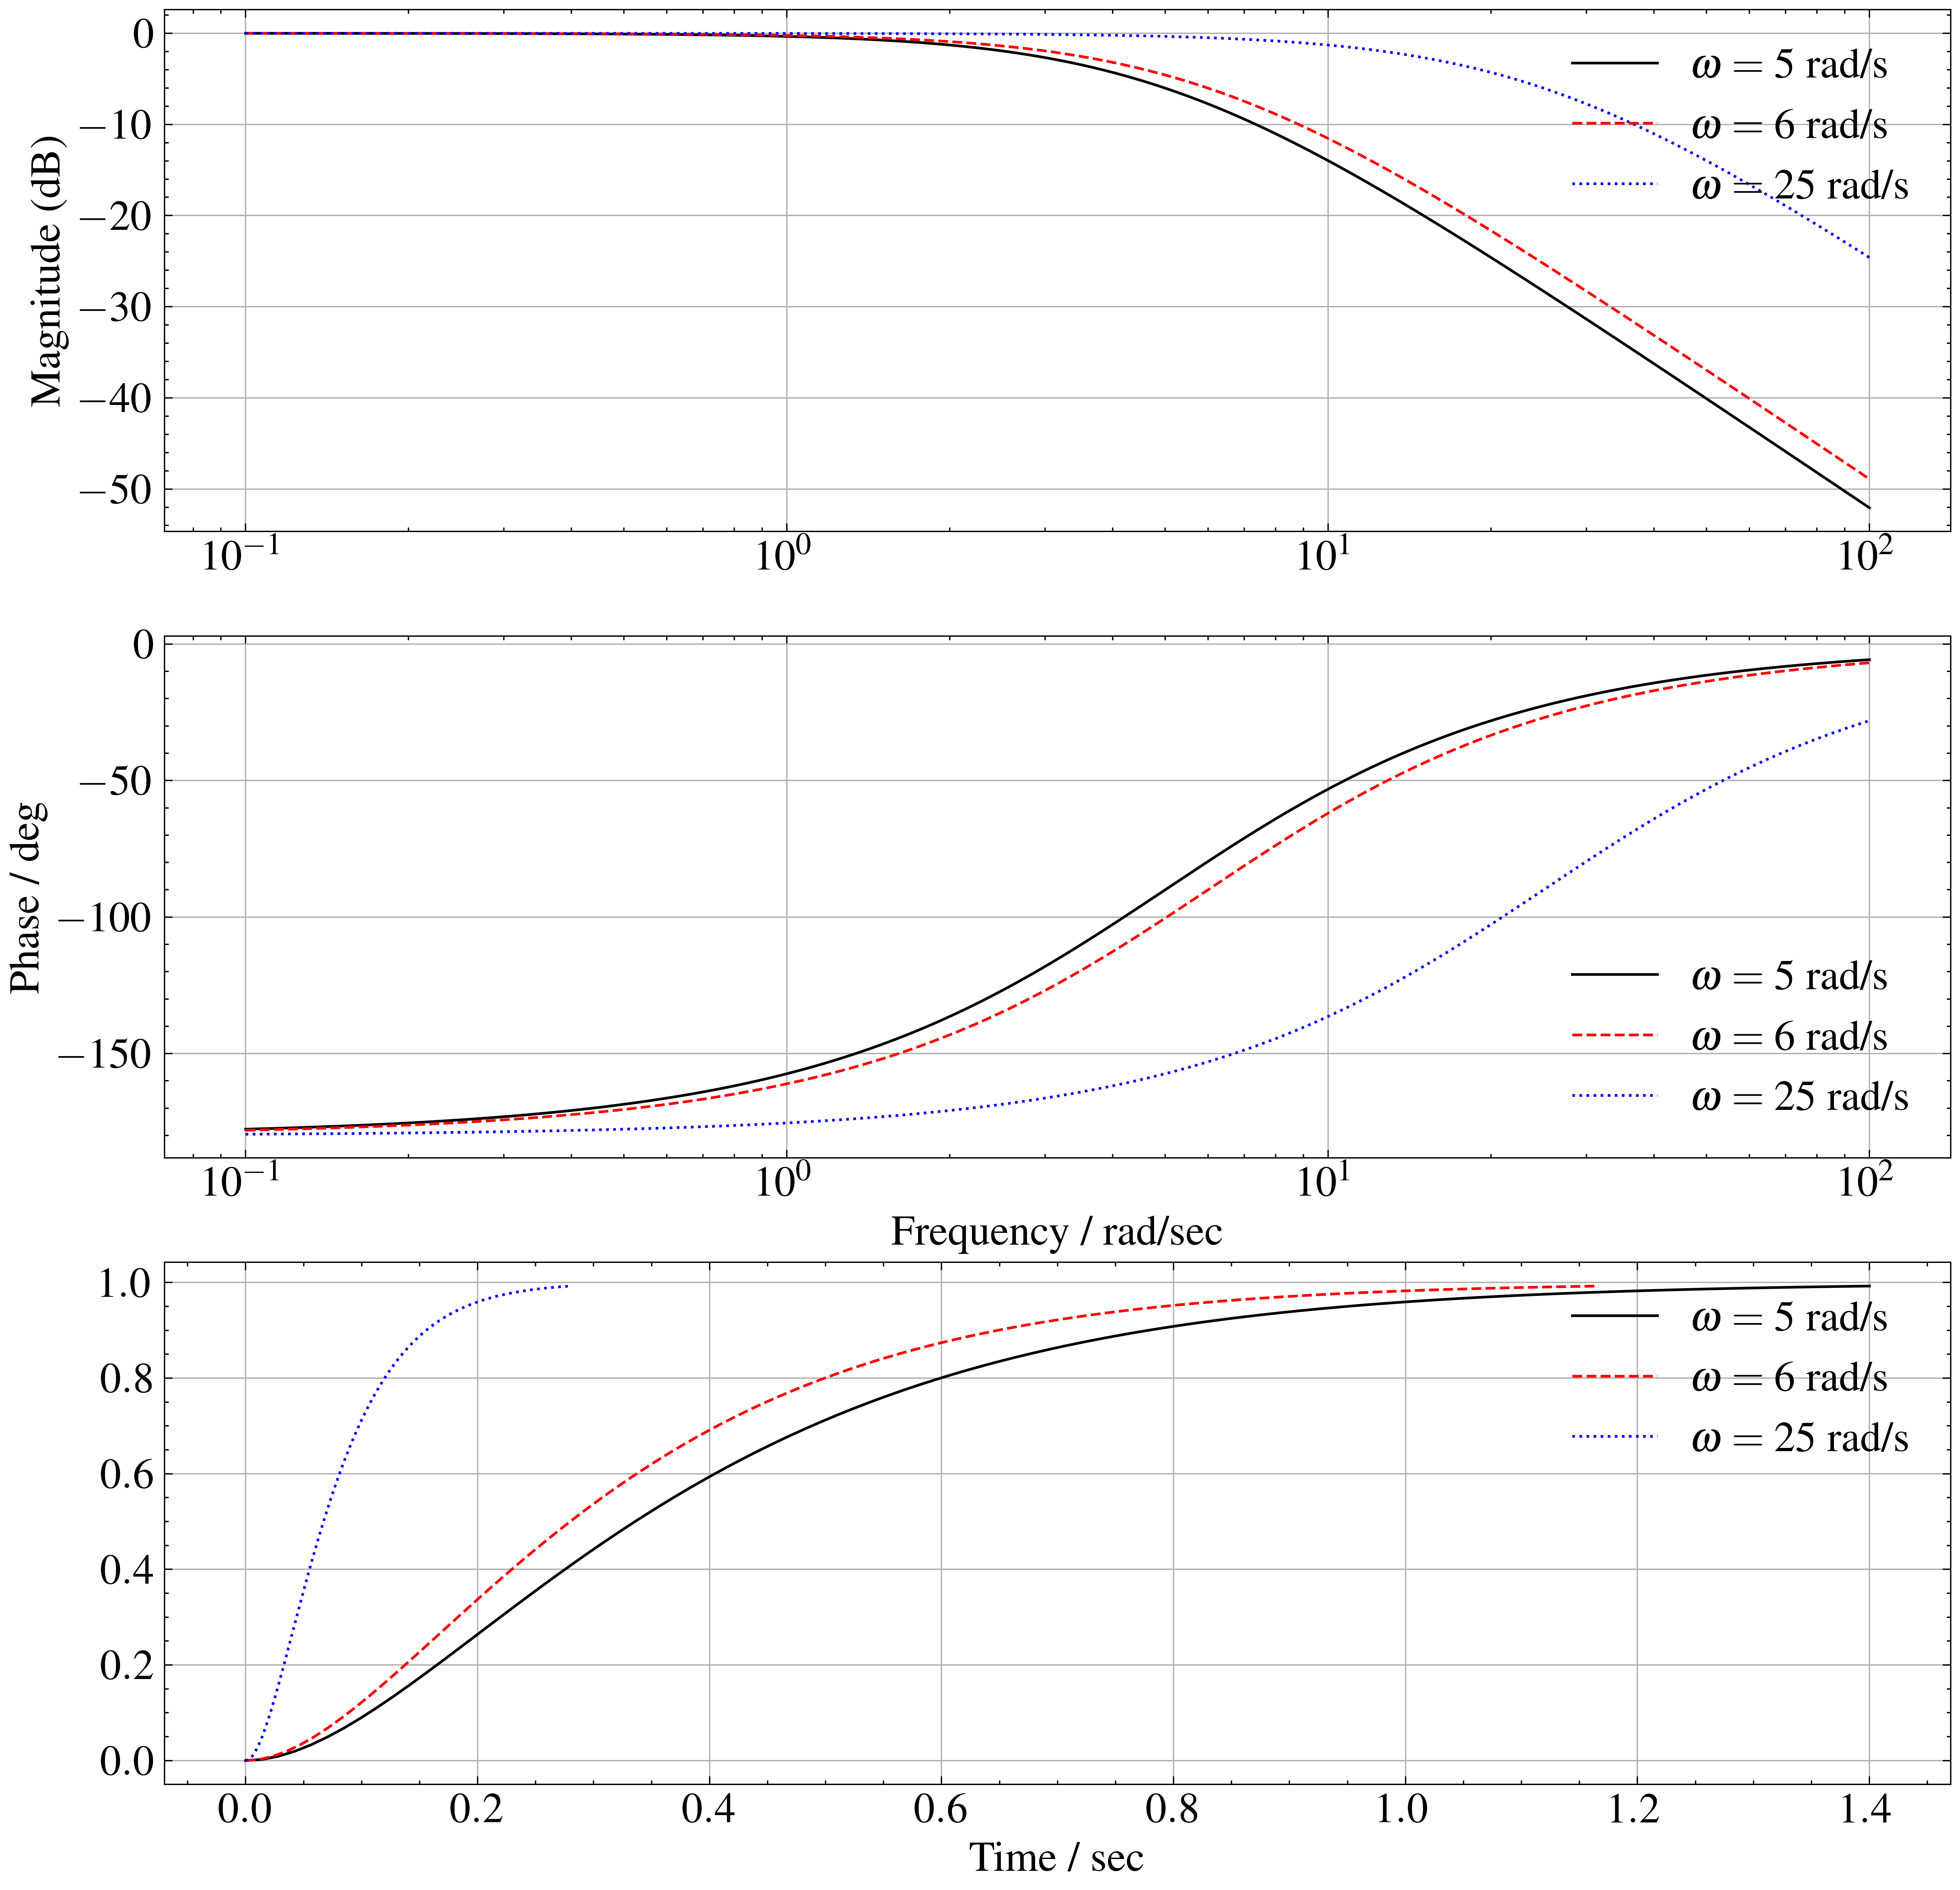
\includegraphics[width=0.8\linewidth]{src/figures/bode-phase-step-ideal-group-zeta/bode-phase-step-ideal-group-zeta-1.0.png}
		\subcaption{$\zeta = 1.0$}\label{fig:bode-phase-step-ideal-group-zeta-1.0}
	\end{subfigure}
	\begin{subfigure}{0.8\linewidth}
		\centering
		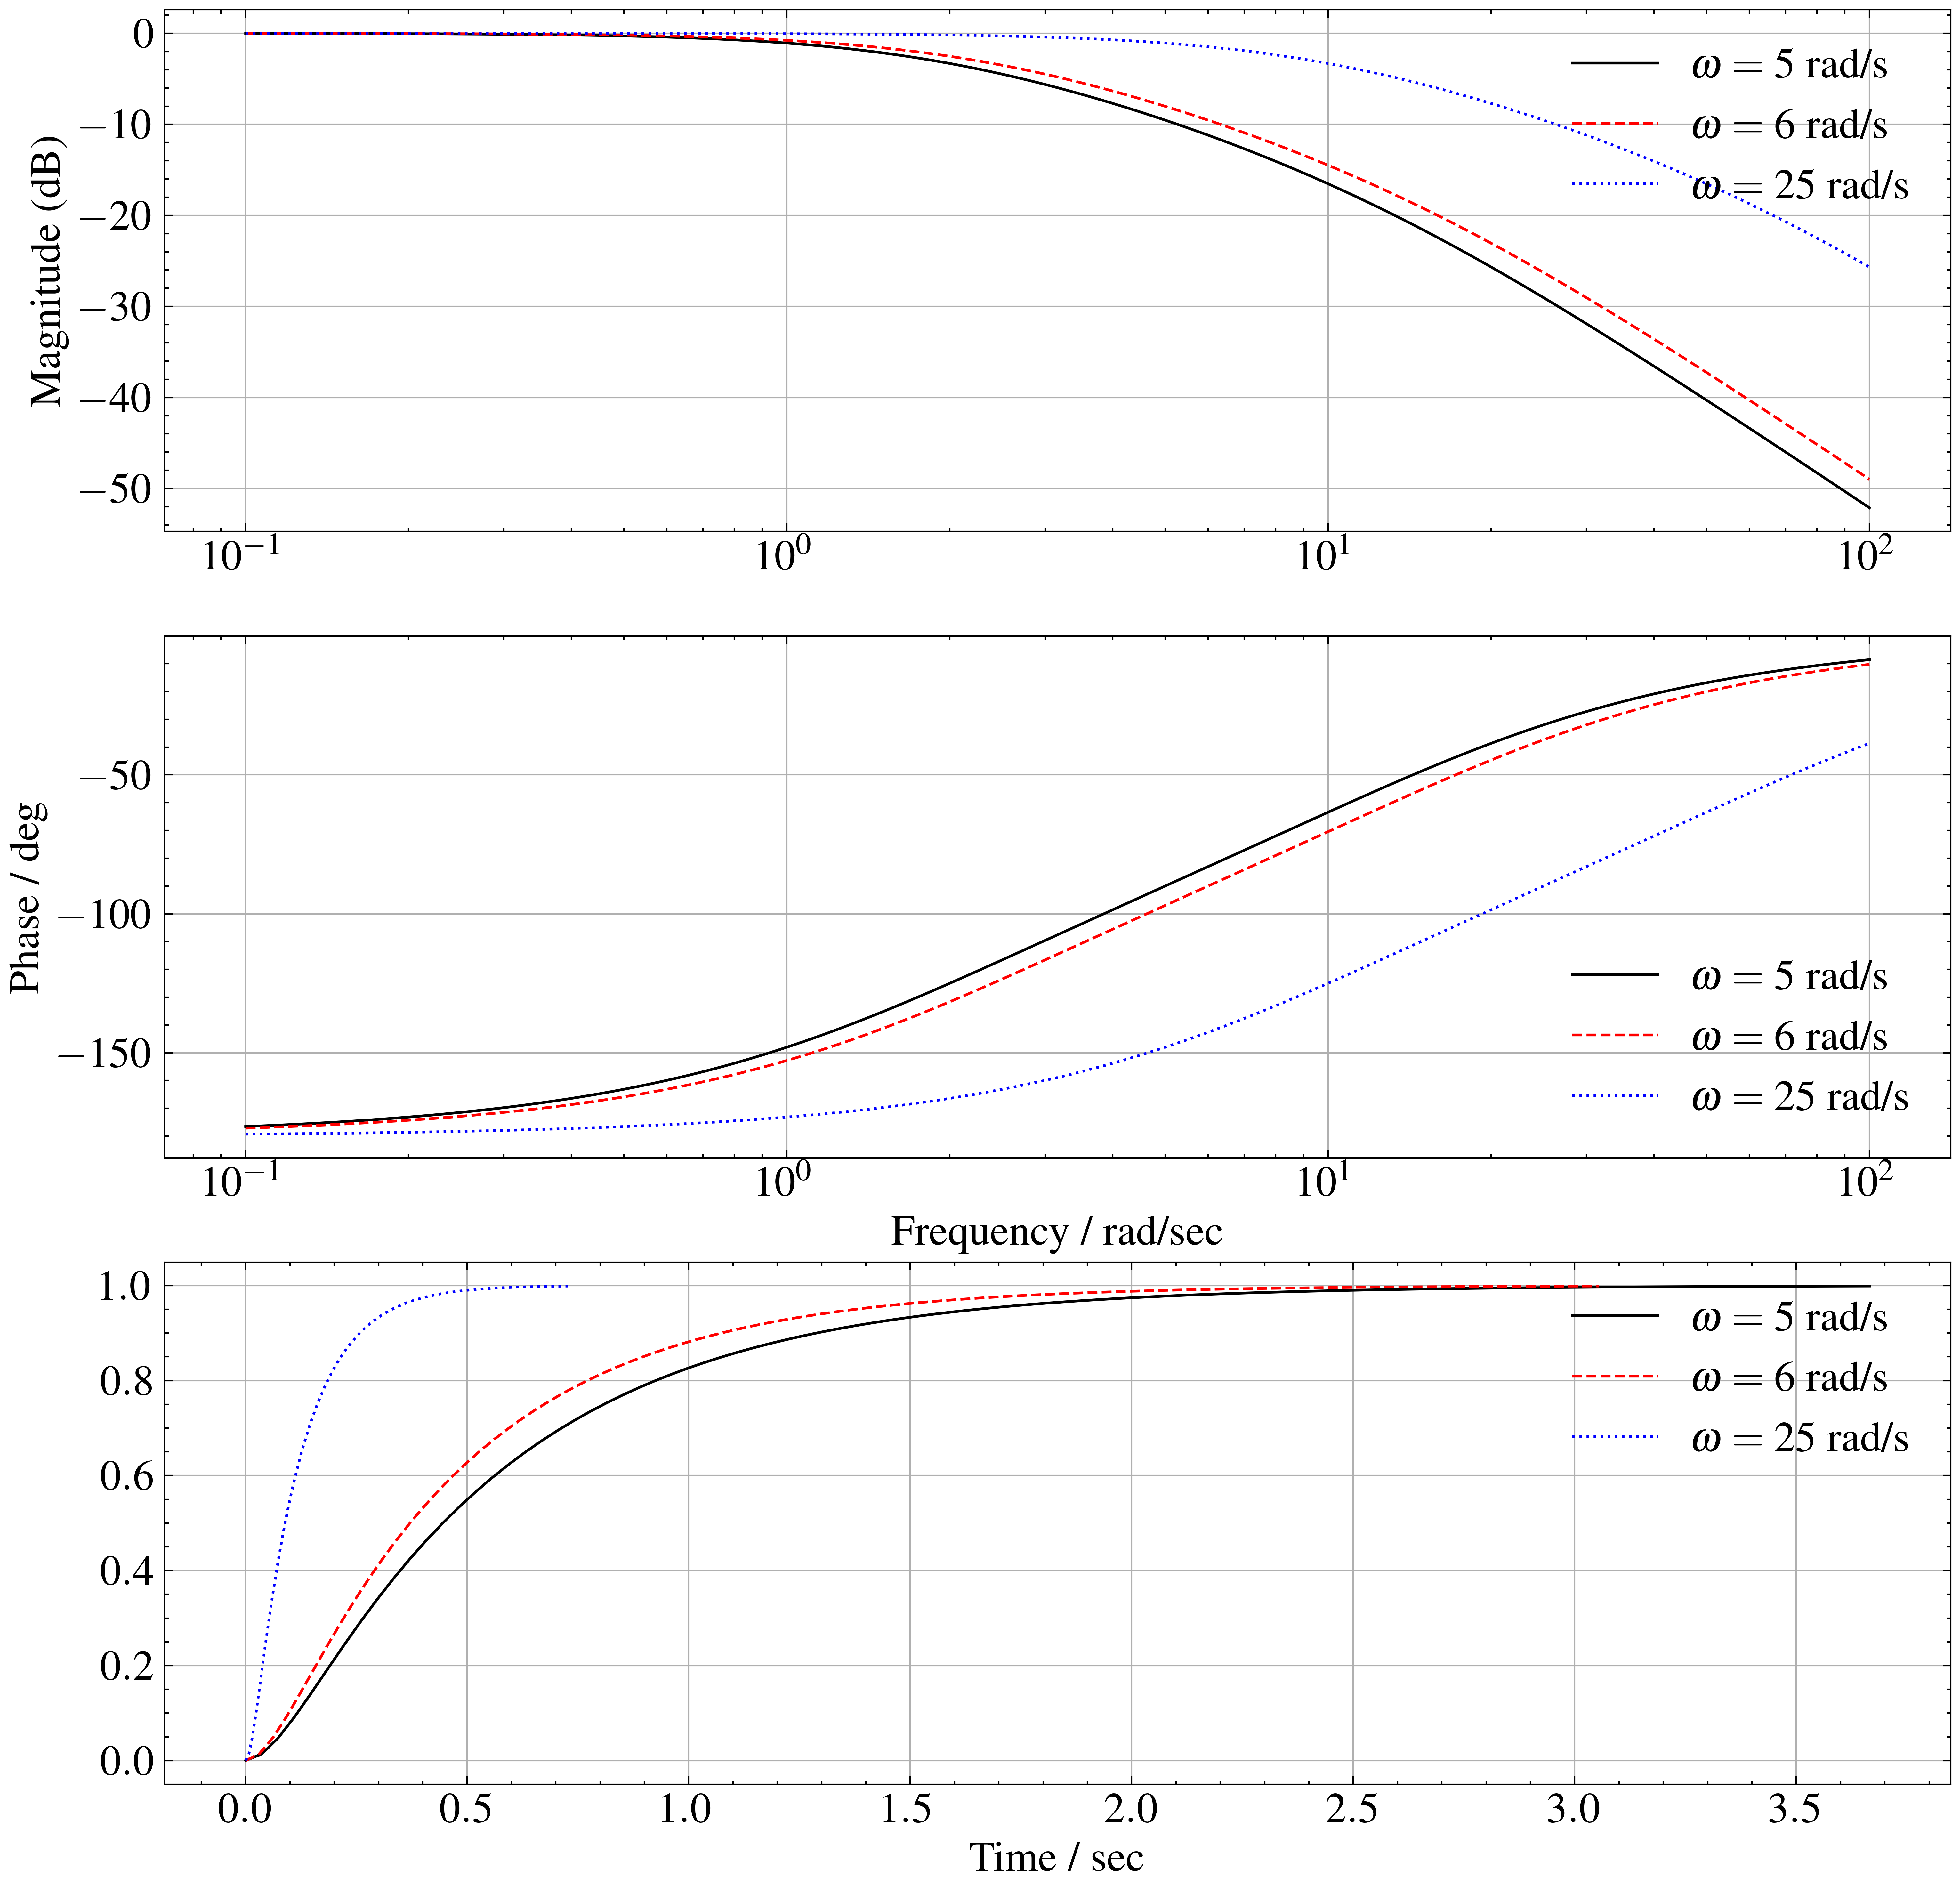
\includegraphics[width=0.8\linewidth]{src/figures/bode-phase-step-ideal-group-zeta/bode-phase-step-ideal-group-zeta-1.5.png}
		\subcaption{$\zeta = 1.5$}\label{fig:bode-phase-step-ideal-group-zeta-1.5}
	\end{subfigure}
	\caption{ある$\zeta$に対して、$\omega$を変化させたときのボード線図とステップ応答(続き1)}
\end{figure}

\begin{figure}
	\centering
	\addtocontents{figure}{-1}
	\begin{subfigure}{0.8\linewidth}
		\setcounter{subfigure}{4}
		\centering
		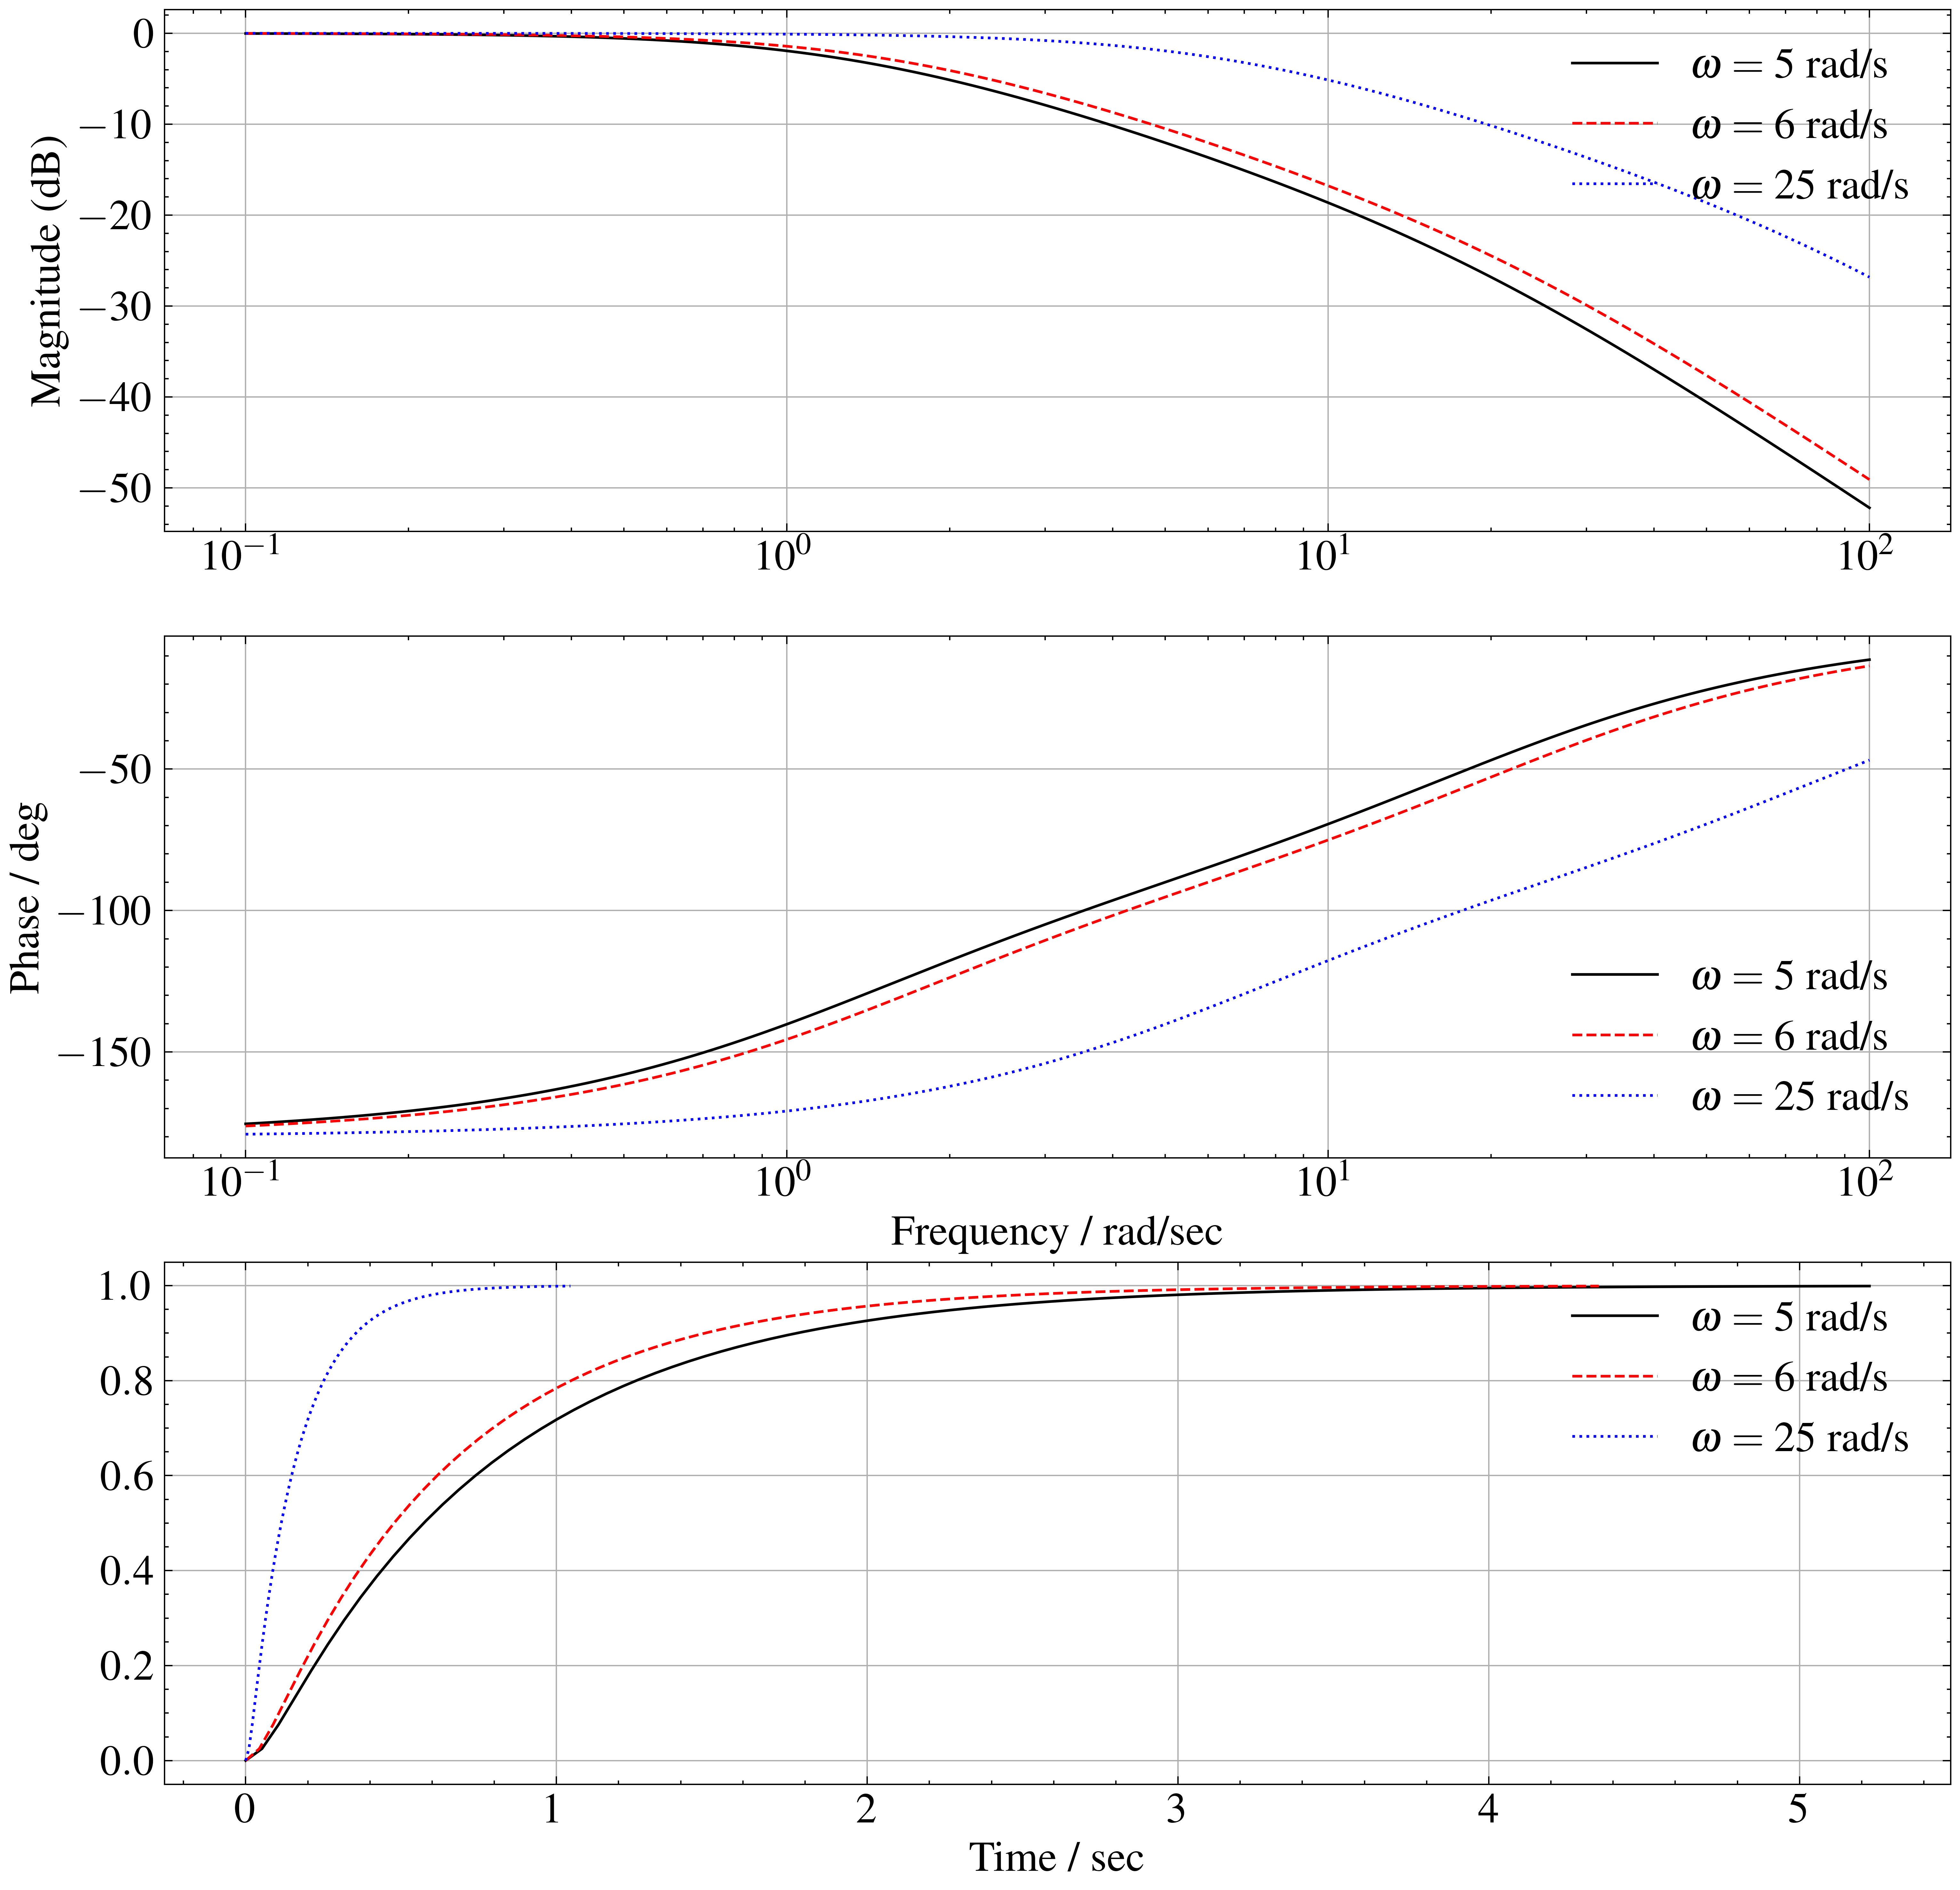
\includegraphics[width=0.8\linewidth]{src/figures/bode-phase-step-ideal-group-zeta/bode-phase-step-ideal-group-zeta-2.0.png}
		\subcaption{$\zeta = 2.0$}\label{fig:bode-phase-step-ideal-group-zeta-2.0}
	\end{subfigure}
	\caption{ある$\zeta$に対して、$\omega$を変化させたときのボード線図とステップ応答(続き2)}
\end{figure}
